\section{Event Tagging}

The HiPO is designed to store data in units of events, where events are collections of data related to each other (usually in time). In nuclear physics
experiments, these events refer to one interaction of a beam particle with the target and record particles produced by the interaction. After the data 
acquisition, the post-processing of the data identifies the number of particles produced and their properties and writes them in the event for further
physics analysis. Specific interactions occur with different frequencies in the physics experiment, and the analysis program analyzing specific physics 
reactions does not analyze every single event but rather requires a specific number of produced particles reconstructed to proceed with the analysis.

In Figure~\ref {fig:event_frequency}, a schematic view is shown of how data can be theoretically distributed in the file. Where event types, are defined by 
a number of rows in the table that lists the particles reconstructed by data processing software. It is evident that for analysis of rare interactions, most of
the data read is not useful and the program spends unnecessary I/O cycles putting pressure on a shared file system and computational resources.

\begin{figure}[h!]
  \begin{center}
    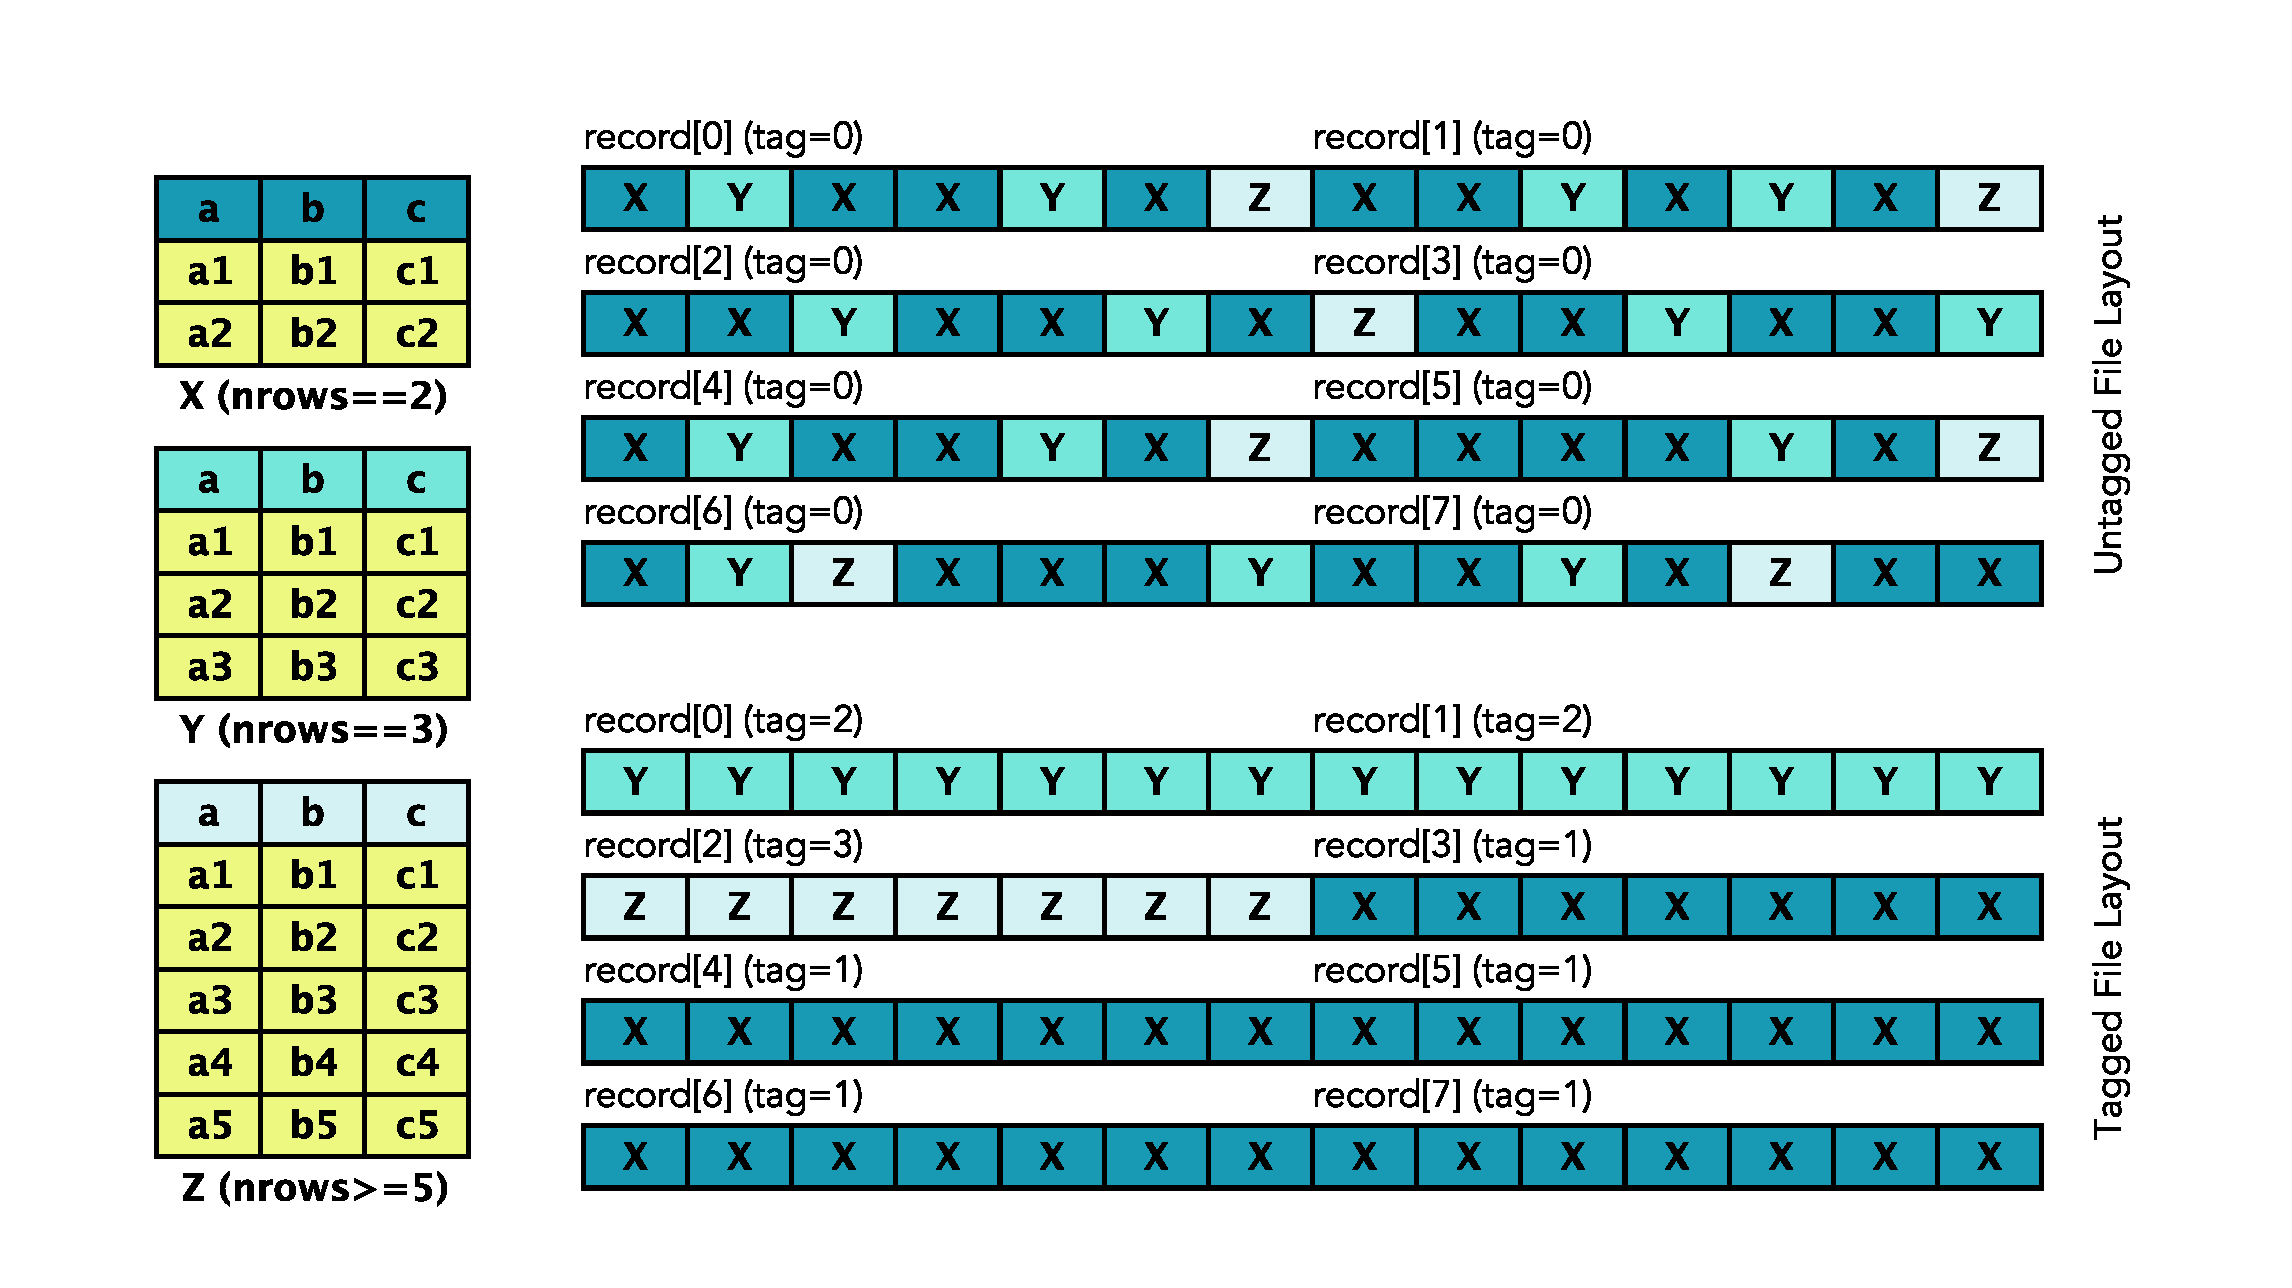
\includegraphics[width=0.85\textwidth]{images/tagged_records.pdf}
 \end{center}
  \caption{Schematic view of the file output for tagged and untagged events. When using the tagged mode of writing a file, events are organized in the records 
  based on the tag of the event, which is assigned by the user depending on the needs.}
 \label{fig:event_frequency}
\end{figure}

To solve this problem, the HiPO data format introduces a tagging feature for storing data. As mentioned before, each record kept in the file contains a unique
tag identifier and this information is stored in the file footer along with the record's positions and sizes. This allows sorting events into separate records during
the writing of the file, which will organize similar events together. The Listing~\ref{lst:write_tagged} shows an example of how to tag events by the number of 
rows contained in a table that lists clusters from the previous example. 

\rule{16.5cm}{0.4pt}
\begin{lstlisting}[language=java, caption=Java example to create and write primitive types into an event, label=lst:write_tagged]
// Writing arrays into an Event
HipoReader r = new HipoReader("myfile.h5");
// using HipoWriter.create() transfers all the dictionary
// and the metadata to the write object
HipoWriter w = HipoWriter.create("taggedfile.h5",r);

Bank[] b = r.getBanks("data::clusters");
Event event = new Event();
while(r.next(event)){
  event.read(b);
  if(b[0].getRows()>=5){
      event.setTag(5);
  } else {
  	event.setTag(b[0].getRows());
  }
  w.addEvent(event);
}
w.close();
\end{lstlisting}

The example code with produce a file where all events with a matching number of rows are grouped together. the events with a specific number of
rows in the "clusters" bank can be read without any overhead of going through the entire file, and example of reading events where the number of
rows in the "clusters" bank are equal to 2 or are larger than 4 as shown in Listing~\ref{lst:read_tagged}.

\rule{16.5cm}{0.4pt}
\begin{lstlisting}[language=java, caption=Java example to sort events in the output file depending on number of rows in the table, label=lst:write_tagged]
// Writing arrays into an Event
HipoReader r = new HipoReader();
r.setTags(2,5); // read only tag=2 and tag=5
r.open("taggedfile.h5");
Bank[] b = r.getBanks("data::clusters");
while(r.nextEvent(b)){
   b[0].show();// print bank content on the screen
}
\end{lstlisting}

Only the bank "data::clusters" containing two rows and/or more than four rows is read in the Listing~\ref{lst:write_tagged}, however, then the event is written to the output file and the entire event with all the banks and nodes is written, but the decision on how to partition a file is based only on one bank. 




%Example usages:
%\begin{verbatim}
%hipo::writer writer("output.file");
%for(int i = 0; i < 12000; i++){
%   hipo::event event = event_provider_next();
%    writer.addEvent(event);
%}
%writer.close();
%\end{verbatim}



%The data from physics experiments is stored in small units called "events", each event contains data related to one physics interaction from a detector. The file consists of a series of events accumulated by the experimental setup during a certain period of time. A HiPO file consists of the following parts:

%- File header: containing file version file length (for consistency check), file footer location, and some other relevant parameters.
%- User header: contains metadata describing the content of the file. In dictionary-driven content contains descriptors of the data 
%stored in the file, the user can add additional information at the creation of the file.
%- Data records: The actual event data grouped and compressed. The size of the data records is configurable at the file creation time. Each record is assigned a user-defined identifier (called tag), which is used to group similar events together.
%- File footer: Contains information about each record in the file, including position, size, and the tag of the record.
%A general structure of the HiPO file is shown in Figure~\ref{hipo_file_structure}.

